%%%%%%%%%%%%%%%%%%%%%%%%%%%%%%%%%%%%%%%%%
% Short Sectioned Assignment
% LaTeX Template
% Version 1.0 (5/5/12)
%
% This template has been downloaded from:
% http://www.LaTeXTemplates.com
%
% Original author:
% Frits Wenneker (http://www.howtotex.com)
%
% License:
% CC BY-NC-SA 3.0 (http://creativecommons.org/licenses/by-nc-sa/3.0/)
%
%%%%%%%%%%%%%%%%%%%%%%%%%%%%%%%%%%%%%%%%%

%----------------------------------------------------------------------------------------
% PACKAGES AND OTHER DOCUMENT CONFIGURATIONS
%----------------------------------------------------------------------------------------

\documentclass[paper=a4, fontsize=11pt]{scrartcl} % A4 paper and 11pt font size

\usepackage[T1]{fontenc} % Use 8-bit encoding that has 256 glyphs
\usepackage{fourier} % Use the Adobe Utopia font for the document - comment this line to return to the LaTeX default
\usepackage[norsk]{babel} 
\usepackage[utf8]{inputenc}
\usepackage{amsmath,amsfonts,amsthm} % Math packages
\usepackage{tikz} % drawing package

\usepackage{sectsty} % Allows customizing section commands
\allsectionsfont{\centering \normalfont\scshape} % Make all sections centered, the default font and small caps

\usepackage{fancyhdr} % Custom headers and footers
\pagestyle{fancyplain} % Makes all pages in the document conform to the custom headers and footers
\fancyhead{} % No page header - if you want one, create it in the same way as the footers below
\fancyfoot[L]{} % Empty left footer
\fancyfoot[C]{} % Empty center footer
\fancyfoot[R]{\thepage} % Page numbering for right footer
\renewcommand{\headrulewidth}{0pt} % Remove header underlines
\renewcommand{\footrulewidth}{0pt} % Remove footer underlines
\setlength{\headheight}{13.6pt} % Customize the height of the header

\numberwithin{equation}{section} % Number equations within sections (i.e. 1.1, 1.2, 2.1, 2.2 instead of 1, 2, 3, 4)
\numberwithin{figure}{section} % Number figures within sections (i.e. 1.1, 1.2, 2.1, 2.2 instead of 1, 2, 3, 4)
\numberwithin{table}{section} % Number tables within sections (i.e. 1.1, 1.2, 2.1, 2.2 instead of 1, 2, 3, 4)

\setlength\parindent{0pt} % Removes all indentation from paragraphs - comment this line for an assignment with lots of text

%---- Listings --------------
\usepackage{color}
\definecolor{light-gray}{gray}{0.95}
\usepackage{listings}

\lstset{ %
language=C,                % choose the language of the code
basicstyle=\footnotesize,       % the size of the fonts that are used for the code
numbers=left,                   % where to put the line-numbers
numberstyle=\footnotesize,      % the size of the fonts that are used for the line-numbers
stepnumber=1,                   % the step between two line-numbers. If it is 1 each line will be numbered
resetmargins=true,              % reset line numbers
numbersep=5pt,                  % how far the line-numbers are from the code
backgroundcolor=\color{white},  % choose the background color. You must add \usepackage{color}
showspaces=false,               % show spaces adding particular underscores
showstringspaces=false,         % underline spaces within strings
showtabs=false,                 % show tabs within strings adding particular underscores
frame=single,           % adds a frame around the code
tabsize=2,          % sets default tabsize to 2 spaces
captionpos=b,           % sets the caption-position to bottom
breaklines=true,        % sets automatic line breaking
breakatwhitespace=false,    % sets if automatic breaks should only happen at whitespace
escapeinside={\%*}{*)}          % if you want to add a comment within your code
}

%----------------------------------------------------------------------------------------
% TITLE SECTION
%----------------------------------------------------------------------------------------

\newcommand{\horrule}[1]{\rule{\linewidth}{#1}} % Create horizontal rule command with 1 argument of height

\title{ 
\normalfont \normalsize 
\textsc{TDT4205 Compilers, NTNU} \\ [25pt] % Your university, school and/or department name(s)
\horrule{0.5pt} \\[0.4cm] % Thin top horizontal rule
\huge Problem Set 2 \\ % The assignment title
\horrule{2pt} \\[0.5cm] % Thick bottom horizontal rule
}

\author{Stian Jensen} % Your name

\date{\normalsize\today} % Today's date or a custom date

\begin{document}

\maketitle % Print the title

%----------------------------------------------------------------------------------------
% PROBLEM 1
%----------------------------------------------------------------------------------------

\section{Regular Languages}

%----------------------------------------------------------------------------------------
\subsection{Part a)}
A possible NFA for the regular expression $a(b|c)d*e$ is:

\begin{center}
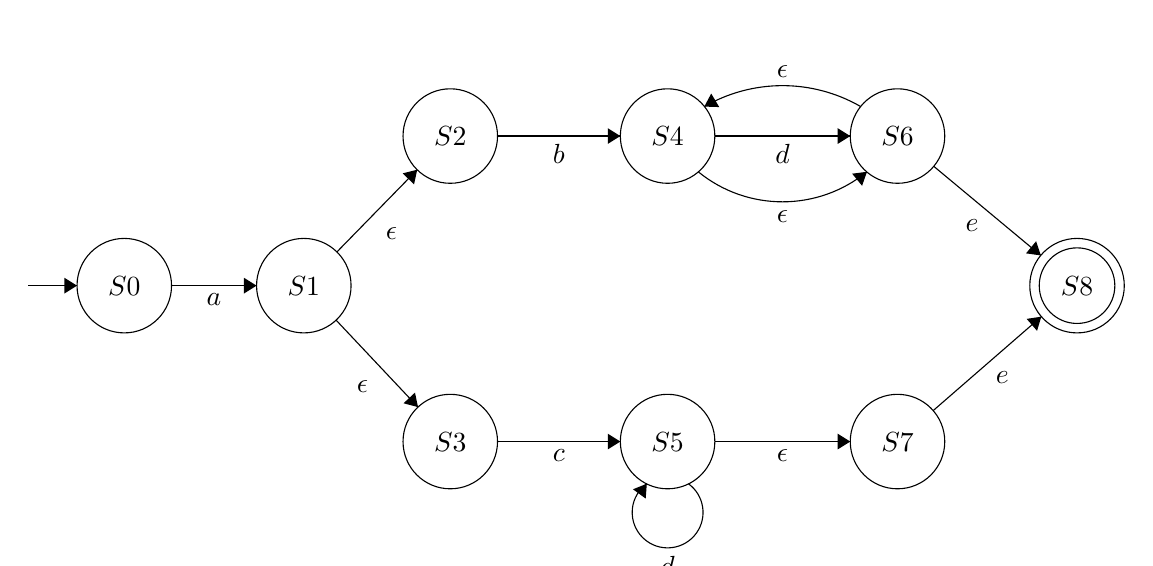
\begin{tikzpicture}[scale=0.2]
\tikzstyle{every node}+=[inner sep=0pt]
\draw [black] (9.5,-27.6) circle (3);
\draw (9.5,-27.6) node {$S0$};
\draw [black] (20.9,-27.6) circle (3);
\draw (20.9,-27.6) node {$S1$};
\draw [black] (30.2,-18.1) circle (3);
\draw (30.2,-18.1) node {$S2$};
\draw [black] (30.2,-37.5) circle (3);
\draw (30.2,-37.5) node {$S3$};
\draw [black] (44,-18.1) circle (3);
\draw (44,-18.1) node {$S4$};
\draw [black] (44,-37.5) circle (3);
\draw (44,-37.5) node {$S5$};
\draw [black] (58.6,-18.1) circle (3);
\draw (58.6,-18.1) node {$S6$};
\draw [black] (58.6,-37.5) circle (3);
\draw (58.6,-37.5) node {$S7$};
\draw [black] (70,-27.6) circle (3);
\draw (70,-27.6) node {$S8$};
\draw [black] (70,-27.6) circle (2.4);
\draw [black] (3.4,-27.6) -- (6.5,-27.6);
\fill [black] (6.5,-27.6) -- (5.7,-27.1) -- (5.7,-28.1);
\draw [black] (12.5,-27.6) -- (17.9,-27.6);
\fill [black] (17.9,-27.6) -- (17.1,-27.1) -- (17.1,-28.1);
\draw (15.2,-28.1) node [below] {$a$};
\draw [black] (23,-25.46) -- (28.1,-20.24);
\fill [black] (28.1,-20.24) -- (27.18,-20.47) -- (27.9,-21.17);
\draw (26.08,-24.32) node [right] {$\epsilon$};
\draw [black] (22.95,-29.79) -- (28.15,-35.31);
\fill [black] (28.15,-35.31) -- (27.96,-34.39) -- (27.23,-35.07);
\draw (25.02,-34.02) node [left] {$\epsilon$};
\draw [black] (33.2,-37.5) -- (41,-37.5);
\fill [black] (41,-37.5) -- (40.2,-37) -- (40.2,-38);
\draw (37.1,-38) node [below] {$c$};
\draw [black] (33.2,-18.1) -- (41,-18.1);
\fill [black] (41,-18.1) -- (40.2,-17.6) -- (40.2,-18.6);
\draw (37.1,-18.6) node [below] {$b$};
\draw [black] (47,-18.1) -- (55.6,-18.1);
\fill [black] (55.6,-18.1) -- (54.8,-17.6) -- (54.8,-18.6);
\draw (51.3,-18.6) node [below] {$d$};
\draw [black] (46.332,-16.231) arc (120.04036:59.95964:9.923);
\fill [black] (46.33,-16.23) -- (47.28,-16.26) -- (46.77,-15.4);
\draw (51.3,-14.4) node [above] {$\epsilon$};
\draw [black] (56.658,-20.366) arc (-50.74625:-129.25375:8.468);
\fill [black] (56.66,-20.37) -- (55.72,-20.49) -- (56.35,-21.26);
\draw (51.3,-22.78) node [below] {$\epsilon$};
\draw [black] (60.9,-20.02) -- (67.7,-25.68);
\fill [black] (67.7,-25.68) -- (67.4,-24.78) -- (66.76,-25.55);
\draw (63.34,-23.34) node [below] {$e$};
\draw [black] (60.87,-35.53) -- (67.73,-29.57);
\fill [black] (67.73,-29.57) -- (66.8,-29.71) -- (67.46,-30.47);
\draw (65.26,-33.04) node [below] {$e$};
\draw [black] (45.323,-40.18) arc (54:-234:2.25);
\draw (44,-44.75) node [below] {$d$};
\fill [black] (42.68,-40.18) -- (41.8,-40.53) -- (42.61,-41.12);
\draw [black] (47,-37.5) -- (55.6,-37.5);
\fill [black] (55.6,-37.5) -- (54.8,-37) -- (54.8,-38);
\draw (51.3,-38) node [below] {$\epsilon$};
\end{tikzpicture}
\end{center}

%----------------------------------------------------------------------------------------
\subsection{Part b)}
The NFA in Figure 1 can be converted to the following DFA.
Equivalent states are denoted by the same state number as in Figure 1.

\begin{center}
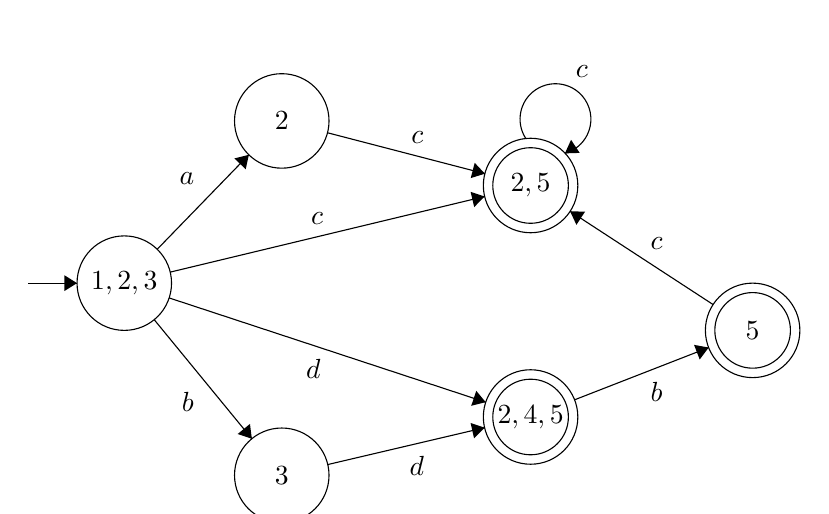
\begin{tikzpicture}[scale=0.2]
\tikzstyle{every node}+=[inner sep=0pt]
\draw [black] (9.5,-27.6) circle (3);
\draw (9.5,-27.6) node {$1,2,3$};
\draw [black] (19.5,-17.3) circle (3);
\draw (19.5,-17.3) node {$2$};
\draw [black] (35.3,-21.4) circle (3);
\draw (35.3,-21.4) node {$2,5$};
\draw [black] (35.3,-21.4) circle (2.4);
\draw [black] (35.3,-36.1) circle (3);
\draw (35.3,-36.1) node {$2,4,5$};
\draw [black] (35.3,-36.1) circle (2.4);
\draw [black] (19.5,-39.8) circle (3);
\draw (19.5,-39.8) node {$3$};
\draw [black] (49.4,-30.6) circle (3);
\draw (49.4,-30.6) node {$5$};
\draw [black] (49.4,-30.6) circle (2.4);
\draw [black] (3.4,-27.6) -- (6.5,-27.6);
\fill [black] (6.5,-27.6) -- (5.7,-27.1) -- (5.7,-28.1);
\draw [black] (11.59,-25.45) -- (17.41,-19.45);
\fill [black] (17.41,-19.45) -- (16.49,-19.68) -- (17.21,-20.37);
\draw (13.97,-20.98) node [left] {$a$};
\draw [black] (12.42,-26.9) -- (32.38,-22.1);
\fill [black] (32.38,-22.1) -- (31.49,-21.8) -- (31.72,-22.77);
\draw (21.74,-23.93) node [above] {$c$};
\draw [black] (22.4,-18.05) -- (32.4,-20.65);
\fill [black] (32.4,-20.65) -- (31.75,-19.96) -- (31.5,-20.93);
\draw (28.11,-18.79) node [above] {$c$};
\draw [black] (35.003,-18.427) arc (213.43723:-74.56277:2.25);
\draw (38.56,-14.56) node [above] {$c$};
\fill [black] (37.48,-19.36) -- (38.42,-19.33) -- (37.87,-18.5);
\draw [black] (12.35,-28.54) -- (32.45,-35.16);
\fill [black] (32.45,-35.16) -- (31.85,-34.44) -- (31.53,-35.39);
\draw (21.51,-32.39) node [below] {$d$};
\draw [black] (11.4,-29.92) -- (17.6,-37.48);
\fill [black] (17.6,-37.48) -- (17.48,-36.54) -- (16.7,-37.18);
\draw (13.94,-35.13) node [left] {$b$};
\draw [black] (22.42,-39.12) -- (32.38,-36.78);
\fill [black] (32.38,-36.78) -- (31.49,-36.48) -- (31.71,-37.45);
\draw (28.07,-38.53) node [below] {$d$};
\draw [black] (46.89,-28.96) -- (37.81,-23.04);
\fill [black] (37.81,-23.04) -- (38.21,-23.9) -- (38.76,-23.06);
\draw (43.3,-25.5) node [above] {$c$};
\draw [black] (38.09,-35.01) -- (46.61,-31.69);
\fill [black] (46.61,-31.69) -- (45.68,-31.52) -- (46.04,-32.45);
\draw (43.3,-33.87) node [below] {$b$};
\end{tikzpicture}
\end{center}

%----------------------------------------------------------------------------------------
\subsection{Part c)}
In C, the syntax for while loops have many variants. Some examples are:
\begin{lstlisting}
// do-while loop
do {
    stuff();
} while(...);

// null loop
while(...);
\end{lstlisting}

The given regex does not take these ways of writing a while loop into account, only the standard way. This means that if you encounter any of these other syntaxes, the result becomes a mess. In both cases the regex will delete everything in its path until it encounters $\{$. After it has encountered that, it will continue removing code until it encounters a $\}$ symbol, and will delete that character as well.

The regular expression could be improved with an addition of either match the regex given in the assignment, but also test if the loop is in the form $while(...) ... ;$. So a regex that matches the keyword while and some noise then a semicolon.

One issue is that we could get a dangeling semicolon on the end of a line. The following code will give a dangeling semicolon, so we need to add that to the first part of the regex.

\begin{lstlisting}
#include <stdio.h>

int main() {
    while(1) if(1) { printf("help! I'm trapped in a printf statement!\n"); };
    return 1;
}
\end{lstlisting}

The new regex will then be.
$$while[\textasciicircum\textbackslash\{]*\textbackslash\{[\textasciicircum\textbackslash\}]*\textbackslash\};?|while.*;$$

A problem now will be that the following code will not be deleted as intended.
\begin{lstlisting}
#include <stdio.h>

int main() {
    while(1) if(1) {
        printf("help! I'm trapped in a printf statement!\n");
        if(1) {
            printf("This will break the regex matching\n");
        }
    };
    return 1;
}
\end{lstlisting}

The end conclusion is that removing this in a regex creates a lot of problems and edge cases. We need to keep account of how many curly braces we have passed to know what scope we are in, and if we are in the while loop or not.
%----------------------------------------------------------------------------------------
% PROBLEM 2
%----------------------------------------------------------------------------------------

\section{Grammars}

\subsection{Part a}

An ambiguous grammar, is a grammar for which there is a string that can have more than one leftmost derivation.

\subsection{Part b}



%----------------------------------------------------------------------------------------

\end{document}
